\section{Multiverso de Barbie}

En el multiverso de Barbie, todos los salarios se leen en número máquina; si esta información se procesa en una máquina que tiene 13 bits para la mantisa, 4 para el exponente y 2 para los signos, resuelva:
\\
Mi Trabajo es Barbie Rappi y el Salario es $252.43$.

\subsection{(1.5 pt) Determine Salario}

Determine cuánto salario en dolares máquina ganarías y qué profesión tendrías según tu cédula si fueras una "Barbie girl". Entregue su procedimiento.
\\

Para convertir el salario de Barbie a su representación binaria, realizamos la conversión tanto para la parte entera como para la parte decimal.
\\

La parte entera de 252 se representa como \(11111100\) y la parte decimal de 0.43 se representa aproximadamente como \(01101\). Por lo tanto, \(252.43\) en binario es aproximadamente \(11111100.01101\).
\\

La notación científica binaria de este número es \(1.1111100.01101\) con un exponente de 7. Sin embargo, con un sesgo de 7 para la representación del exponente en la máquina, sumamos 7 al exponente para obtener \(1110\) en binario.
\\

La representación final de este número en la máquina de Barbie es \(00\) (para los signos) seguido de \(1110\) (para el exponente) y luego \(1111100011010\) (para la mantisa).

\subsection{(0.5) Salario Real}
Si asumimos que el salario real es el dado por la máquina transformado a decimal y el aproximado el de la tabla, encuentre la exactitud y la dispersión para su profesión.
\\

Para calcular la exactitud y la dispersión, primero encontramos el error absoluto y relativo entre el valor real y el valor aproximado.

\textbf{1. Error Absoluto (EA):}
\[ \text{EA} = |252.43 - 252.40625| \]
\[ \text{EA} = 0.02375 \]

\textbf{2. Error Relativo (ER):}
\[ \text{ER} = \frac{\text{EA}}{252.43} \]
\[ \text{ER} \approx 0.00009407 \]

\textbf{3. Exactitud:}
Dado que la exactitud es simplemente el valor real menos el error absoluto, obtenemos:
\[ \text{Exactitud} \approx 252.40625 \]

\textbf{4. Dispersión:}
\[ \text{Dispersión} = \text{ER} \times 100\% \]
\[ \text{Dispersión} \approx 0.009407\% \]


\subsection{(1.5) Intervalos}

Ahora que Barbie es empoderada y factura bastante, Ken se siente preocupado ya que cree que con su salario no logrará que Barbie vuelva a aceptarlo.  Ken requiere entonces identificar para qué intervalos de salario se encuentra bien condicionada la siguiente función. Ayúdale a Ken a encontrar estos intervalos, ya que él es medio atembado.

\[ f(x) = \frac{1}{ln(x^{2}) + C(0)}\]

donde x está en miles de dolares y  C es el dígito final de su cédula. Entregue su procedimiento.
\\

Para determinar en qué intervalos la función \( f(x) = \frac{1}{\ln(x^2)} \) está bien condicionada, consideramos su derivada:

\[ f'(x) = \frac{-\frac{2}{x}}{(\ln(x^2))^2} \]

La función tendrá puntos críticos y posiblemente intervalos mal condicionados donde su derivada es grande en valor absoluto, y está bien condicionada donde la derivada es pequeña en valor absoluto. Sin embargo, observamos que la derivada tiene singularidades en \( x=0 \) y donde \( \ln(x^2) = 0 \), es decir, \( x = 1 \) y \( x = e \).

Ahora bien, el número de condición de una función \( f \) en un punto \( x \) está dado por:

\[ K(x) = x \cdot \left| \frac{f'(x)}{f(x)} \right| \]

Para nuestra función \( f(x) = \frac{1}{\ln(x^2)} \), la derivada es:

\[ f'(x) = \frac{-\frac{2}{x}}{(\ln(x^2))^2} \]

El número de condición es entonces:

\[ K(x) = x \cdot \left| \frac{\frac{-\frac{2}{x}}{(\ln(x^2))^2}}{\frac{1}{ln(x)^2}} \right| \]

Para determinar dónde la función está bien o mal condicionada, se observa el valor absoluto de \( K(x) \). Si \( |K(x)| \) es significativamente mayor que 1, la función puede ser mal condicionada en ese punto.

\begin{figure}[H]
    \centering
    \begin{subfigure}[b]{\textwidth}
        \centering
        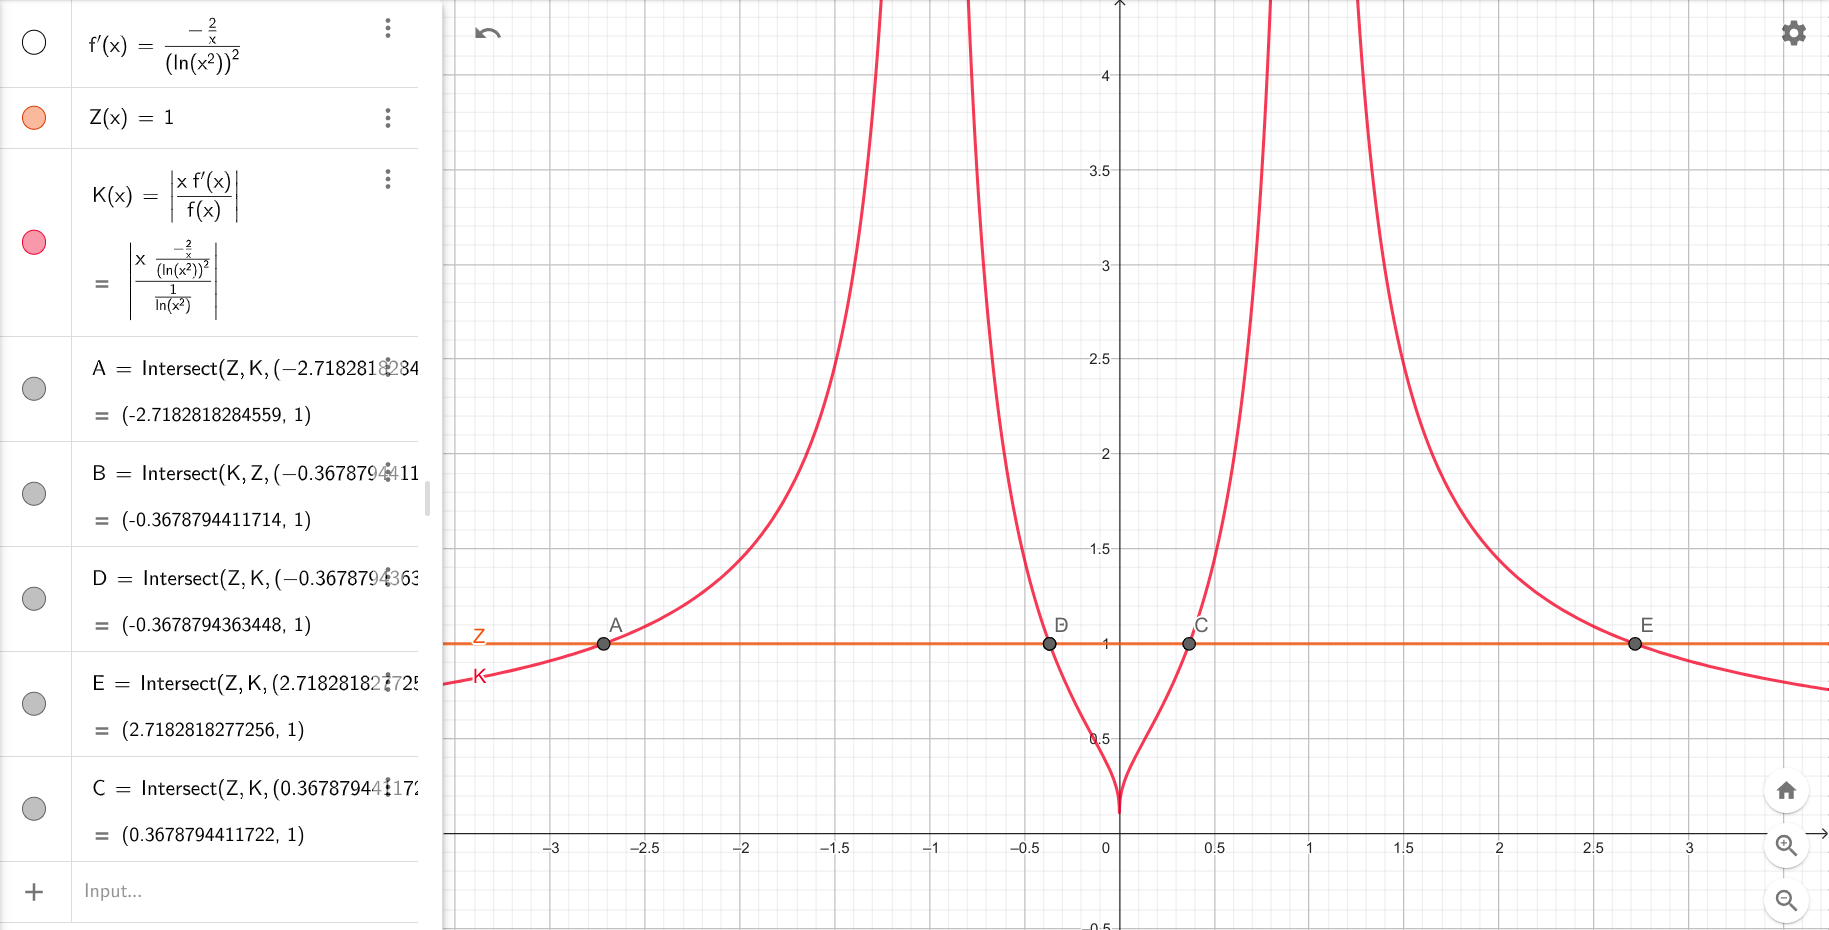
\includegraphics[width=\textwidth]{Figures/0. General/1.3.png}
        \caption{Gráfica K(x) con sus intervalos}
        \label{fig: Grafica K(x)}
    \end{subfigure}
\end{figure}

Del Intersecto $A (-2.7182818284559, 1)$ al $B (-0.3678794411714, 1)$ la función $K(x)$
es mayor que 1, y para el intersecto entre $C (0.3678794411722, 1)$ y
$D (2.7182818277256, 1)$ también es mayor que 1, pero por fuera de estos
intervalos la función $K(x)$ da menor que 1.

\subsection{(0.5) Salario de Ken}

Si el salario de Ken es el mismo calculado en el primer punto, determine si Ken se encuentra bien o mal condicionado para estar con Barbie y explique ¿por qué?

Para el punto 4, usando el salario de Ken como \( x = 252.40625 \times 10^{-3} = 0.25240625 \), determinamos si está bien o mal condicionado evaluando el número de condición \( K(x) \) en \( x = 0.25240625 \):

\[ K(0.25240625) = 0.25240625 \cdot \left| \frac{\frac{-\frac{2}{0.25240625}}{(\ln(0.25240625^2))^2}}{\frac{1}{ln(0.25240625^2)}} \right| \]

Según los intervalos mencionados anteriormente, 0.25240625 no se encuentra en los rangos donde \( K(x) \) es mayor que 1. Por lo tanto, Ken está bien condicionado para estar con Barbie.
